\documentclass[UKenglish]{uioexam}
\usepackage{amsmath}
\usepackage{amssymb}
\usepackage{tabularx}

\usepackage{url}
\usepackage{hyperref}
\hypersetup{
    colorlinks=true,
    linkcolor=blue,
    filecolor=magenta,      
    urlcolor=blue,
    pdftitle={Overleaf Example},
    pdfpagemode=FullScreen,
    }
\newcommand{\answerbox}{\fbox{\phantom{M}}}
\usepackage{setspace}
\usepackage{minted}
\usepackage{graphicx}
\usepackage[T1]{fontenc}
\usepackage[french]{babel,textcomp}
\usepackage{multicol}
\dato{7 décembre 2023, 08h-09h}
\emne{\textsc{}}{}
\tid{}{}
\usepackage{eso-pic}
\newcommand{\abox}[2]{\makebox[#1][l]{#2 \rightarrowfill}}  


\begin{document}
    \AddToShipoutPictureFG*{
    \AtPageUpperLeft{\put(-50,-50){\makebox[\paperwidth][r]{\huge20/20}}}  
    }%
\onehalfspacing
\section[REN]{\small(4 points)}
Dans la phrase suivante, soulignez toutes les entités nommées :

\textit{\underline{Emmanuel Macron}, né \underline{le 21 décembre 1977} à \underline{Amiens}, est \underline{président de la France}}
\\~\\
$\ast$ \textbf{Remarque} : \textit{la France} est une entité nommée de lieu qui est imbriquée à l'intérieur de l'entité nommée désignant le titre (\textit{président de la France}).

\section[Regex]{\small(1 point)}
Parmi les options ci-dessous, choisissez celle(s) qui correspond(ent) à (aux) expression(s) régulière(s) valide(s) :

\begin{choicelist}[]
   \makebox[0pt][l]{$\square$}\raisebox{0.15ex}{\hspace{0.1em}$\checkmark$} \texttt{\^{}jour}\\

    \makebox[0pt][l]{$\square$}\raisebox{0.15ex}{\hspace{1em}☐}
    \texttt{[[\^{}jour}\\

    \makebox[0pt][l]{$\square$}\raisebox{0.15ex}{\hspace{1em}☐}
    \texttt{[a-zA-Z0-9\_])}\\

   \makebox[0pt][l]{$\square$}\raisebox{0.15ex}{\hspace{0.1em}$\checkmark$} \texttt{[a-zA-Z0-9\_]}\\

\end{choicelist}
\section[OCR]{\small(1 point)}
Comment s’appelle l’étape initiale d’une chaîne de traitement d’\textsc{OCR} ?

\begin{choicelist}[]
   \makebox[0pt][l]{$\square$}\raisebox{0.15ex}{\hspace{1em}☐} exportation\\

    \makebox[0pt][l]{$\square$}\raisebox{0.15ex}{\hspace{1em}☐}
    prédiction\\

    \makebox[0pt][l]{$\square$}\raisebox{0.15ex}{\hspace{1em}☐}
    transcription\\

   \makebox[0pt][l]{$\square$}\raisebox{0.15ex}{\hspace{0.1em}$\checkmark$} segmentation\\

\end{choicelist}


\section[Transkribus]{\small(1 point)}
Remplissez le blanc avec le mot approprié :

Transkribus est une plateforme de la \underline{reconnaissance / transcription} automatique des textes.

\section[Acquisition]{\small(2 points)}
L’illustration suivante représente un exemple de (plusieurs réponses possibles) :
\begin{choicelist}[]
   \makebox[0pt][l]{$\square$}\raisebox{0.15ex}{\hspace{1em}☐} l’annotation des entités nommées suivant le format \textsc{BIO}\\

    \makebox[0pt][l]{$\square$}\raisebox{0.15ex}{\hspace{0.1em}$\checkmark$}
    la cartographie des entités nommées\\

    \makebox[0pt][l]{$\square$}\raisebox{0.15ex}{\hspace{1em}☐}
    la campagne d’évaluation de la reconnaissance d’entités nommées\\

   \makebox[0pt][l]{$\square$}\raisebox{0.15ex}{\hspace{0.1em}$\checkmark$} la désambiguïsation des entités nommées
   
   \begin{figure}[H]
    \centering
    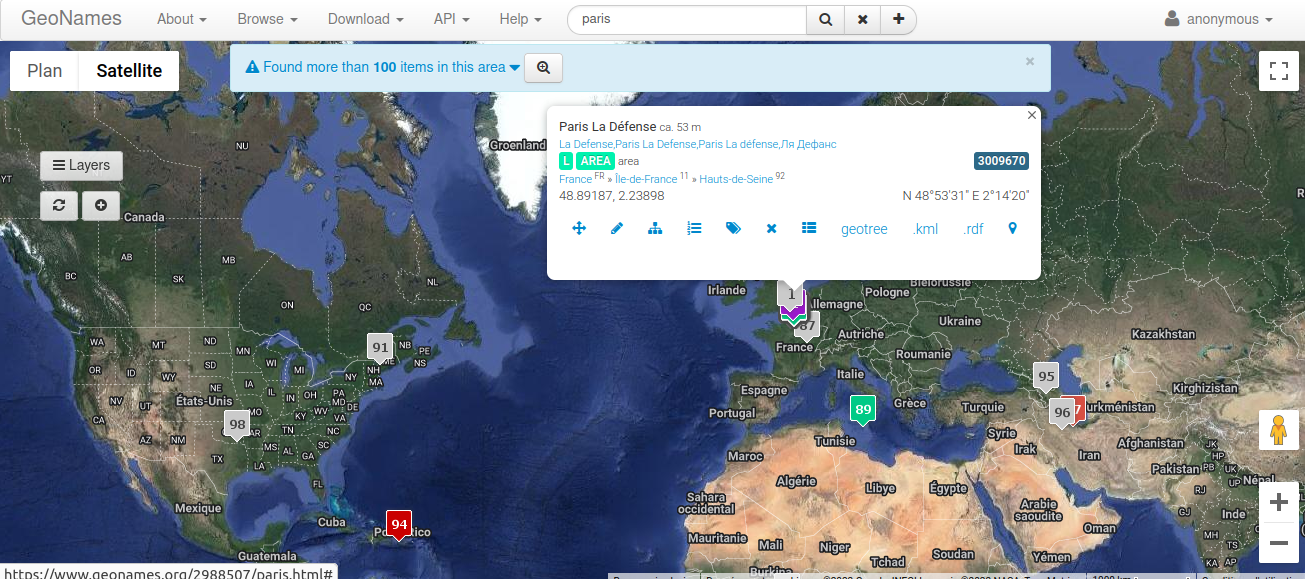
\includegraphics[width=1\textwidth]{img/geonames.png}
    % \caption{a nice plot}
    \label{fig:mesh1}
\end{figure}


\end{choicelist}

\section[Regex_2]{\small(1 point)}
Quel est l’intérêt d’utilisation des expressions régulières ?\\

\fbox{\begin{minipage}{33em}
Les expressions régulières, aussi dénommées \textit{regex}, fournissent un moyen concis et flexible pour la correspondance de chaînes de caractères dans un texte, telles que des caractères particuliers, mots ou motifs (patrons) de caractères.
\end{minipage}}

\section[Règles · OCR]{\small(2 points)}
Répondez par \textsc{Vrai} (\textsc{V}) ou \textsc{Faux} (\textsc{F}) aux phrases suivantes :\\
\newcounter{abc}
\renewcommand{\theabc}{\stepcounter{abc}\alph{abc}}
\newcommand{\answerbox}{\fbox{\phantom{M}}}
\begin{document}
\def\arraystretch{2}% increase vertical spacing
\noindent\begin{tabularx}{\textwidth}{cXcc}
 & & V & F\\
% (\theabc) & Les éléments cachés se reconnaissent au point précédant leur nom. & \answerbox & \answerbox\\
% (\theabc) & La commande \mintinline{bash}{ls -a} liste uniquement les noms des fichiers et des répertoires visibles dans le répertoire courant. & \answerbox & \answerbox\\
(\theabc) & L’approche à base de règles pour effectuer certaines tâches de \textsc{TAL} nécessite un entraînement d’un modèle. & \makebox[0pt][c]{$\square$}{\hspace{0em}} & \makebox[-1pt][l]{$\square$}\raisebox{0.15ex}{\hspace{0.15em}$\checkmark$} \\
(\theabc) & Généralement, les logiciels d’\textsc{OCR} / \textsc{HTR} permettent
d’exporter des transcriptions dans différents formats. & \makebox[-1pt][l]{$\square$}\raisebox{0.15ex}{\hspace{0.15em}$\checkmark$} & \makebox[0pt][c]{$\square$}{\hspace{0em}}
\end{tabularx}

% \section[Chemins relatifs et absolus]{\small(2 points)}
% \begin{enumerate}
% %     \item Quel est le type de chemin
% % \mintinline{bash}{dossier/page.html} ? \makebox[5.3cm]{\hrulefill}
%     \item Quel est le type de chemin
% \mintinline{bash}{/home/page.html} ? \makebox[4cm]{\hrulefill}
%     \item Que désigne l'élément \texttt{.} (point) étant donné le chemin \mintinline{bash}{./dossier/page.html} ?  \makebox[6cm]{\hrulefill}.
%     % \item Étant donné le chemin \mintinline{bash}{../dossier/page.html}, l'élément \texttt{../} signifie que la page est cherchée à partir du répertoire \makebox[5.9cm]{\hrulefill}.
%     \end{enumerate}
\section[Regex_3]{\small(2 points)}
Étant donné la phrase \textit{Je suis en train de réviser pour mon 2\textsuperscript{ème} partiel}, formulez les regex qui permettent de capturer les mots suivants :
\begin{enumerate}
    \item \textit{2\textsuperscript{ème}} : \underline{\texttt{\textbackslash{dème}}} ou \underline{\texttt{[0-9]ème}}
    \item \textit{Je} : \underline{\texttt{[A-Z]e}}
    
\end{enumerate}

\section[Voyant_Tools]{\small(3 points)}\label{voyant}
\begin{enumerate}
\item Chargez le corpus \href{https://icampus.univ-paris3.fr/mod/resource/view.php?id=639612}{\textit{Le tour du monde en quatre-vingts jours}} (utilisé lors de la séance du 23 novembre 2023, \og{}Reconnaissance d'entités nommées\fg{}) dans \href{https://voyant-tools.org/}{Voyant Tools} depuis votre ordinateur ;
   \begin{figure}[H]
    \centering
    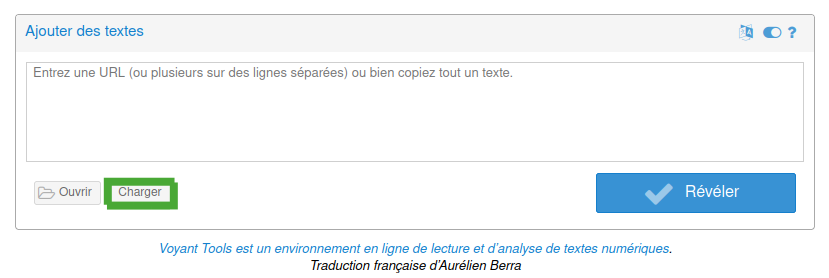
\includegraphics[width=0.8\textwidth]{img/charger.png}
    % \caption{a nice plot}
    \label{fig:mesh1}
\end{figure}

\item Combien de \textit{tokens} et de \textit{types} ce corpus contient-il ?
   \begin{figure}[H]
    \centering
    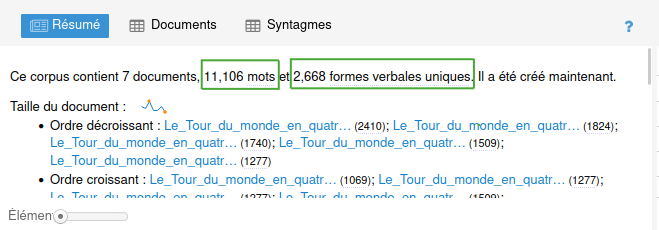
\includegraphics[width=0.8\textwidth]{img/tokens_types.png}
    % \caption{a nice plot}
    \label{fig:mesh1}
\end{figure}

Tokens : \underline{11 106}

Types : \underline{2 668}

\item Quelle est la fréquence absolue du mot \texttt{fogg} ? \underline{107}
   \begin{figure}[H]
    \centering
    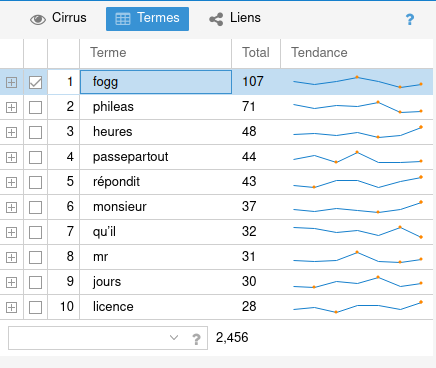
\includegraphics[width=0.6\textwidth]{img/freq_absolue.png}
    % \caption{a nice plot}
    \label{fig:mesh1}
\end{figure}
\end{enumerate}

\section[Tanagra]{\small(3 points)}
\begin{enumerate}
\item Dirigez-vous vers la page de l’outil \href{https://obtic.sorbonne-universite.fr/tanagra/map}{Tanagra}.
   \begin{figure}[H]
    \centering
    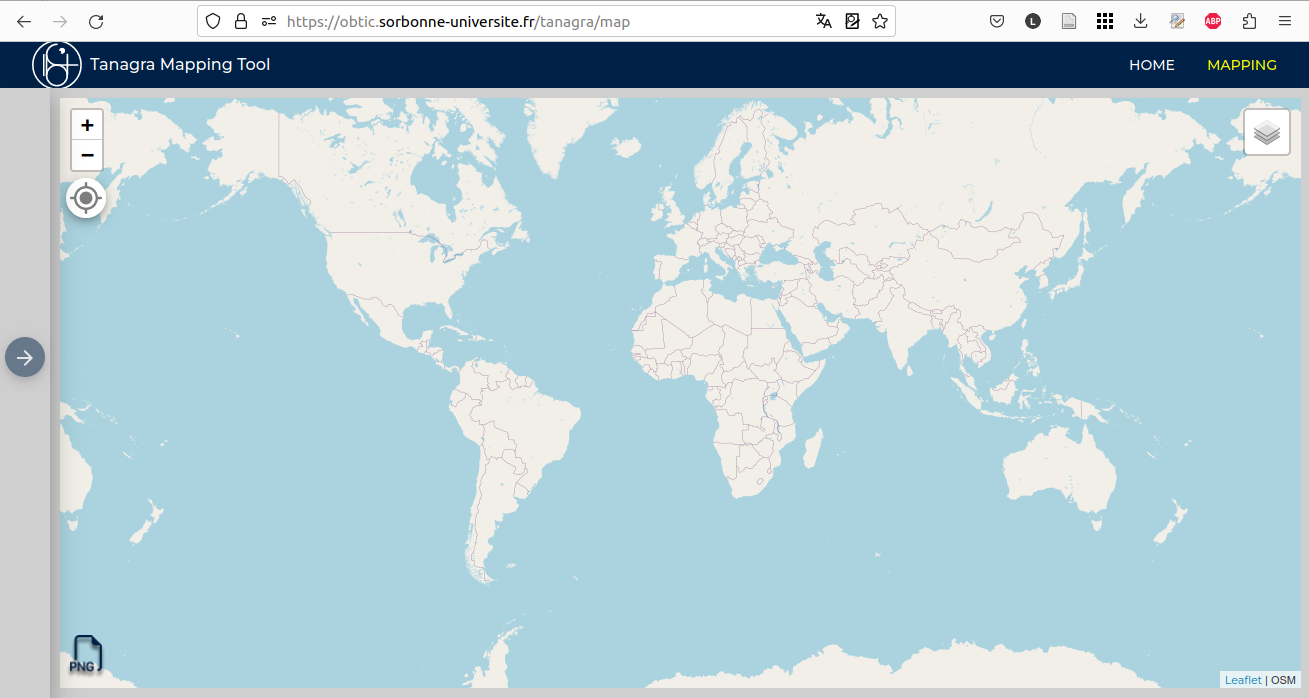
\includegraphics[width=0.8\textwidth]{img/tanagra.png}
    % \caption{a nice plot}
    \label{fig:mesh1}
\end{figure}
\item Sélectionnez \texttt{French\_lg} comme modèle de reconnaissance d’entités nommées :
   \begin{figure}[H]
    \centering
    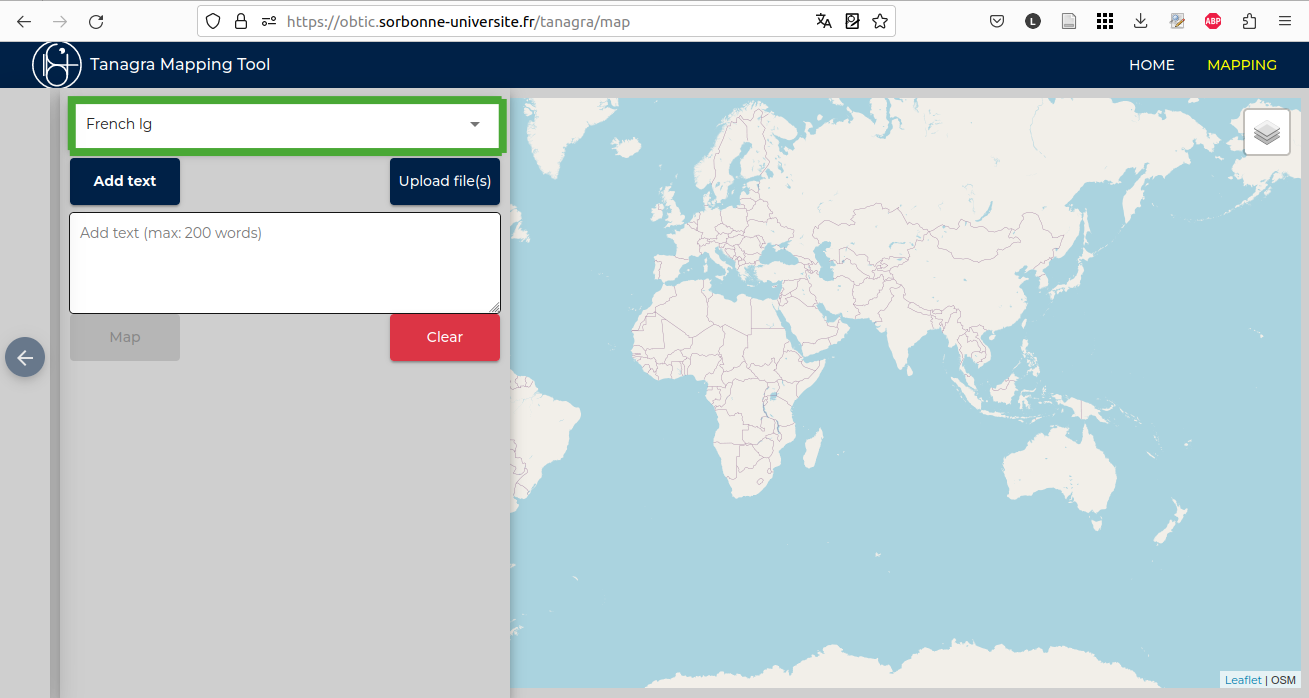
\includegraphics[width=0.8\textwidth]{img/spacy.png}
    % \caption{a nice plot}
    \label{fig:mesh1}
\end{figure}


et chargez le même corpus que dans la question \ref{voyant}}.
   \begin{figure}[H]
    \centering
    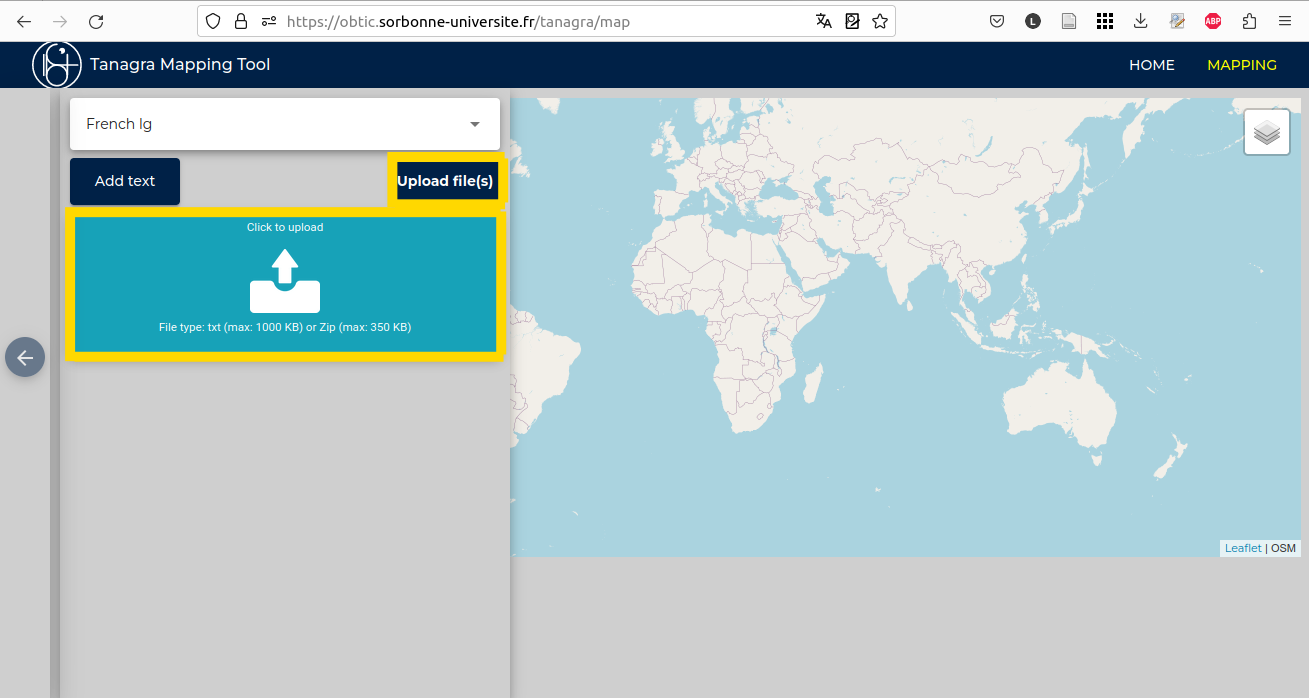
\includegraphics[width=0.8\textwidth]{img/import.png}
    % \caption{a nice plot}
    \label{fig:mesh1}
\end{figure}

\item Parmi les entités nommées récupérées par Tanagra, en trouvez-vous une localisée en Espagne ? Si oui, laquelle ? 
   \begin{figure}[H]
    \centering
    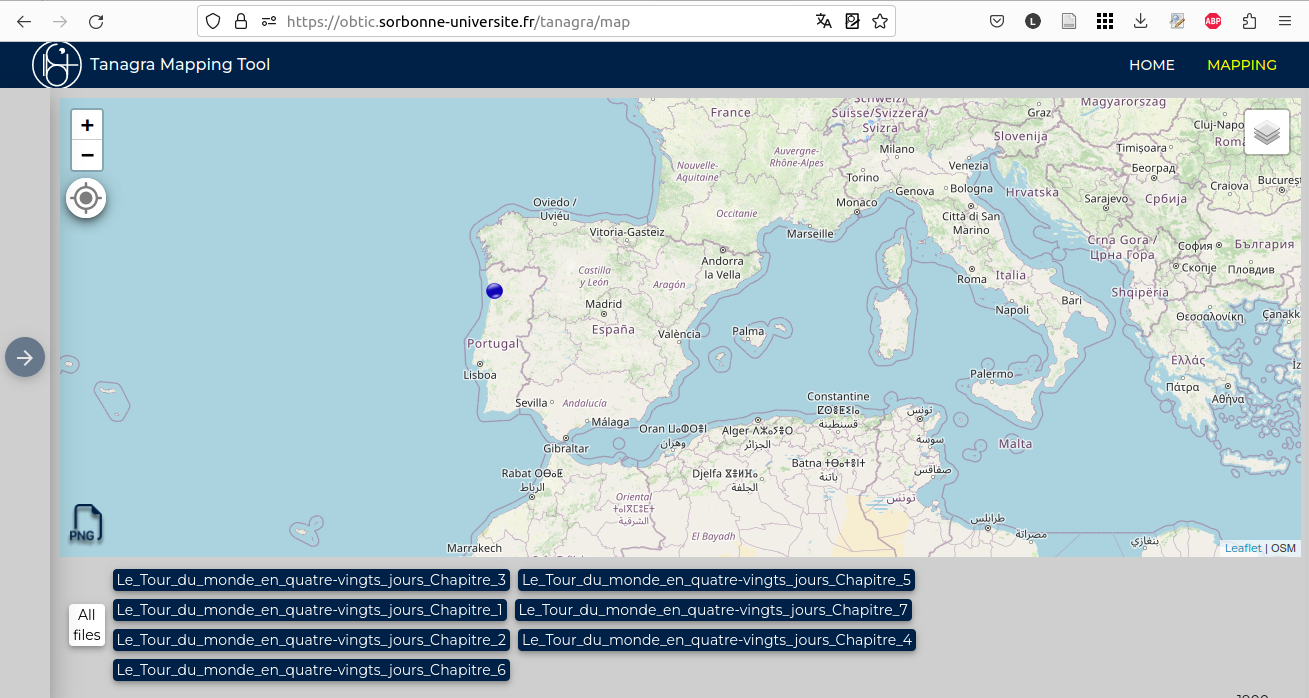
\includegraphics[width=0.8\textwidth]{img/espagne.png}
    % \caption{a nice plot}
    \label{fig:mesh1}
\end{figure}
\end{enumerate}
\fbox{\begin{minipage}{33em}
Non, aucune entité nommée localisée en Espagne n'a été récupérée.
\end{minipage}}

\end{document}